% Options for packages loaded elsewhere
\PassOptionsToPackage{unicode}{hyperref}
\PassOptionsToPackage{hyphens}{url}
%
\documentclass[
]{article}
\usepackage{amsmath,amssymb}
\usepackage{lmodern}
\usepackage{ifxetex,ifluatex}
\ifnum 0\ifxetex 1\fi\ifluatex 1\fi=0 % if pdftex
  \usepackage[T1]{fontenc}
  \usepackage[utf8]{inputenc}
  \usepackage{textcomp} % provide euro and other symbols
\else % if luatex or xetex
  \usepackage{unicode-math}
  \defaultfontfeatures{Scale=MatchLowercase}
  \defaultfontfeatures[\rmfamily]{Ligatures=TeX,Scale=1}
\fi
% Use upquote if available, for straight quotes in verbatim environments
\IfFileExists{upquote.sty}{\usepackage{upquote}}{}
\IfFileExists{microtype.sty}{% use microtype if available
  \usepackage[]{microtype}
  \UseMicrotypeSet[protrusion]{basicmath} % disable protrusion for tt fonts
}{}
\makeatletter
\@ifundefined{KOMAClassName}{% if non-KOMA class
  \IfFileExists{parskip.sty}{%
    \usepackage{parskip}
  }{% else
    \setlength{\parindent}{0pt}
    \setlength{\parskip}{6pt plus 2pt minus 1pt}}
}{% if KOMA class
  \KOMAoptions{parskip=half}}
\makeatother
\usepackage{xcolor}
\IfFileExists{xurl.sty}{\usepackage{xurl}}{} % add URL line breaks if available
\IfFileExists{bookmark.sty}{\usepackage{bookmark}}{\usepackage{hyperref}}
\hypersetup{
  hidelinks,
  pdfcreator={LaTeX via pandoc}}
\urlstyle{same} % disable monospaced font for URLs
\usepackage{graphicx}
\makeatletter
\def\maxwidth{\ifdim\Gin@nat@width>\linewidth\linewidth\else\Gin@nat@width\fi}
\def\maxheight{\ifdim\Gin@nat@height>\textheight\textheight\else\Gin@nat@height\fi}
\makeatother
% Scale images if necessary, so that they will not overflow the page
% margins by default, and it is still possible to overwrite the defaults
% using explicit options in \includegraphics[width, height, ...]{}
\setkeys{Gin}{width=\maxwidth,height=\maxheight,keepaspectratio}
% Set default figure placement to htbp
\makeatletter
\def\fps@figure{htbp}
\makeatother
\setlength{\emergencystretch}{3em} % prevent overfull lines
\providecommand{\tightlist}{%
  \setlength{\itemsep}{0pt}\setlength{\parskip}{0pt}}
\setcounter{secnumdepth}{-\maxdimen} % remove section numbering
\ifluatex
  \usepackage{selnolig}  % disable illegal ligatures
\fi

\author{}
\date{}

\begin{document}

\hypertarget{header-n0}{%
\section{arxiv文献泛读20210125-27}\label{header-n0}}

\hypertarget{header-n2}{%
\subsubsection{\texorpdfstring{\href{./2101.08798.pdf}{Revealing the
cosmic reionisation history with fast radio bursts in the era of Square
Kilometre
Array}}{Revealing the cosmic reionisation history with fast radio bursts in the era of Square Kilometre Array}}\label{header-n2}}

https://arxiv.org/abs/2101.08798

details

Authors: Tetsuya Hashimoto, Tomotsugu Goto, Ting-Yi Lu, Alvina Y. L. On,
Daryl Joe D. Santos, Seong Jin Kim, Ece Kilerci Eser, Simon C.-C. Ho,
Tiger Y.-Y. Hsiao, Leo Y.-W. Lin\\
Comments: Accepted for publication in MNRAS. A summary video is
available at
\href{https://www.youtube.com/watch?v=uis6h_cBnpE\&feature=youtu.be}{this
https URL}

Revealing the cosmic reionisation history is at the frontier of
extragalactic astronomy. The power spectrum of the cosmic microwave
background (CMB) polarisation can be used to constrain the reionisation
history. Here we propose a CMB-independent method using fast radio
bursts (FRBs) to directly measure the ionisation fraction of the
intergalactic medium (IGM) as a function of redshift. FRBs are new
astronomical transients with millisecond timescales. Their dispersion
measure (DMIGM) is an indicator of the amount of ionised material in the
IGM. Since the differential of DMIGM against redshift is proportional to
the ionisation fraction, our method allows us to directly measure the
reionisation history without any assumption on its functional shape. As
a proof of concept, we constructed mock non-repeating FRB sources to be
detected with the Square Kilometre Array, assuming three different
reionisation histories with the same optical depth of Thomson
scattering. We considered three cases of redshift measurements: (A)
spectroscopic redshift for all mock data, (B) spectroscopic redshift for
10\% of mock data, and (C) redshift estimated from an empirical relation
of FRBs between their time-integrated luminosity and rest-frame
intrinsic duration. In all cases, the reionisation histories are
consistently reconstructed from the mock FRB data using our method. Our
results demonstrate the capability of future FRBs in constraining the
reionisation history.

\begin{itemize}
\item
  利用FRB研究宇宙再电离演化
\end{itemize}

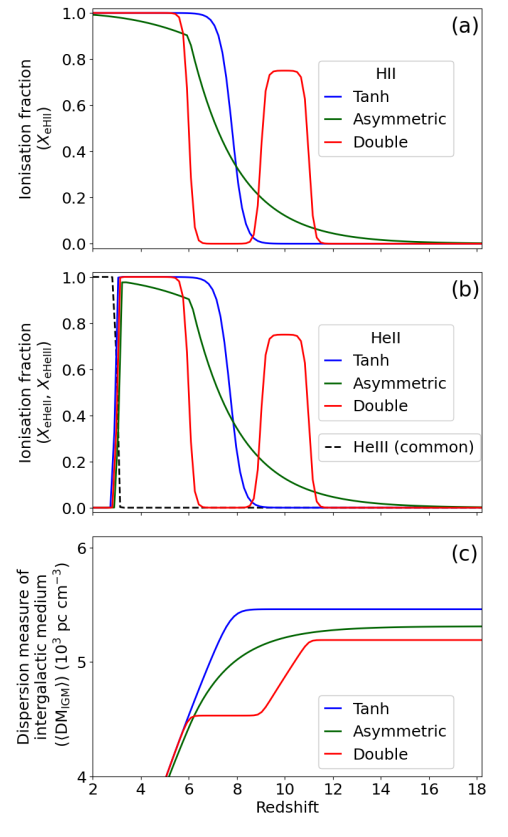
\includegraphics{/home/liuxing/git/Astro101/weekly_news/20210125-27/2101.08798_fig1.png}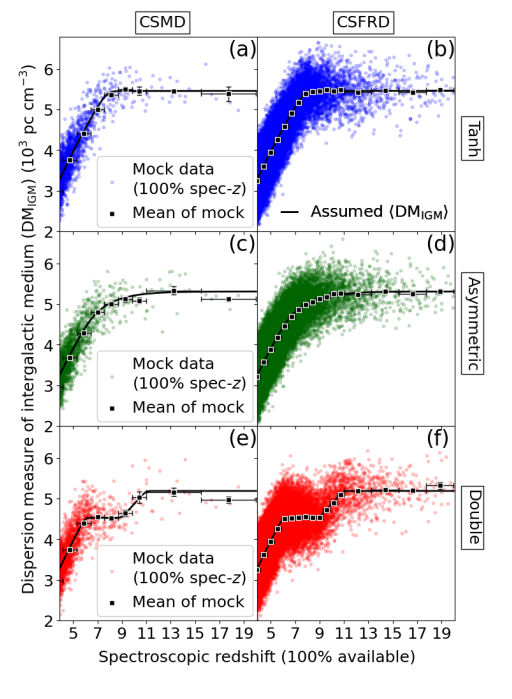
\includegraphics{/home/liuxing/git/Astro101/weekly_news/20210125-27/2101.08798_fig3.png}

\hypertarget{header-n14}{%
\subsubsection{\texorpdfstring{\href{./2101.09694.pdf}{Spectroscopic
monitoring of the candidate tidal disruption event in
F01004-2237}}{Spectroscopic monitoring of the candidate tidal disruption event in F01004-2237}}\label{header-n14}}

https://arxiv.org/abs/2101.09694

details

Authors: Giacomo Cannizzaro, Peter G. Jonker, Daniel Mata-Sánchez\\
Comments: 9 pages, 3 figures, 2 tables. Accepted for publication on ApJ
on January 22, 2021

We present results of spectroscopic monitoring observations of the
Ultra-Luminous Infra Red Galaxy F01004-2237. This galaxy was observed to
undergo changes in its optical spectrum, detected by comparing a
spectrum from 2015 with one from 2000. These changes were coincident
with photometric brightening. The main changes detected in the optical
spectrum are enhanced He II λ4686 emission and the appearance of He I
λ3898,λ5876 emission lines. The favoured interpretation of these changes
was that of a tidal disruption event (TDE) happening in 2010. However,
subsequent work suggested that these changes are caused by another
hitherto unknown reason related to variations in the accretion rate in
the active galactic nucleus (AGN). Our optical spectroscopic monitoring
observations show that the evolution of the He lines is in line with the
evolution seen in TDEs and opposite of what observed from reverberation
mapping studies of AGNs, renewing the discussion on the interpretation
of the flare as a TDE.

\begin{itemize}
\item
  超亮红外星系F01004-2237
  在2015年的光谱与在2000年的光谱相比发生了改变,主要变化是增强的He II
  λ4686 发射线 以及 He I λ3898,λ5876发射线的出现。
\item
  此变化也与其测光增亮相一致。
\item
  较有可能的解释是该变化由发生在2010年的TDE事件导致,但后续的一些工作表明这些变化是由与活动星系核中吸积率的变化相关的原因导致的。
\item
  作者对该源的光谱跟踪观测表明,He线的演化与已知TDE中观察到的演化一致,而与在AGN相关研究(reverberation
  mapping studies)中观察到的不一致。
\item
  因此这个耀发仍有可能是一个TDE。
\end{itemize}

\begin{center}\rule{0.5\linewidth}{0.5pt}\end{center}

\begin{itemize}
\item
  TDE的光谱演化应该是怎样的?AGN光谱应该是怎样的?
\item
  为什么开始用TDE解释光谱变化?
\item
  为什么否定TDE的解释而用AGN相关解释?
\item
  为什么现在又转而支持TDE解释而否定AGN解释?
\end{itemize}

\begin{center}\rule{0.5\linewidth}{0.5pt}\end{center}

\begin{itemize}
\item
  Tadhunter et al. (2017)使用TDE解释观测上的变化\\
  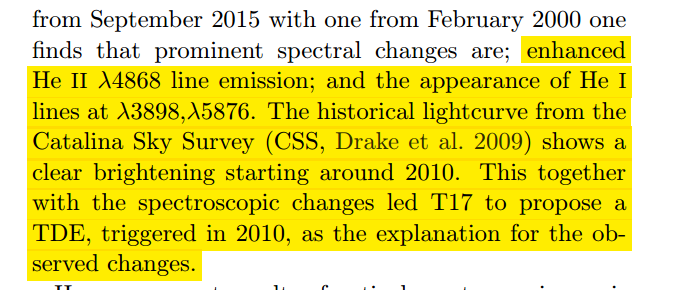
\includegraphics{/home/liuxing/git/Astro101/weekly_news/20210125-27/2101.09694_sa1.png}
\item
  作者支持TDE的理由,以及TDE光谱演化的特征\\
  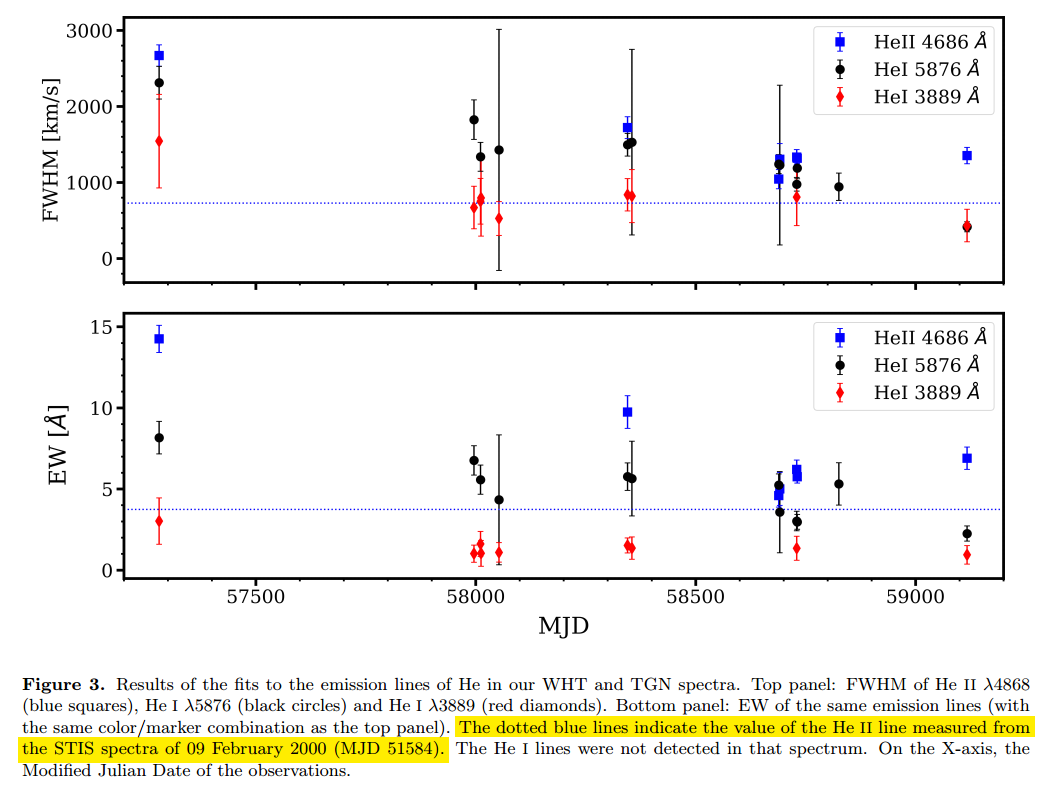
\includegraphics{/home/liuxing/git/Astro101/weekly_news/20210125-27/2101.09694_fig3.png}

  \begin{itemize}
  \item
    1.宽He线是TDE的普遍特征,特别是 He II
    λ4686,尽管根据\href{https://www.nature.com/articles/s41550-018-0661-3.pdf}{Trakhtenbrot
    et al. 2019},大部分TDE的He线宽度要大于F01004-2237光谱中的He宽度。\\
    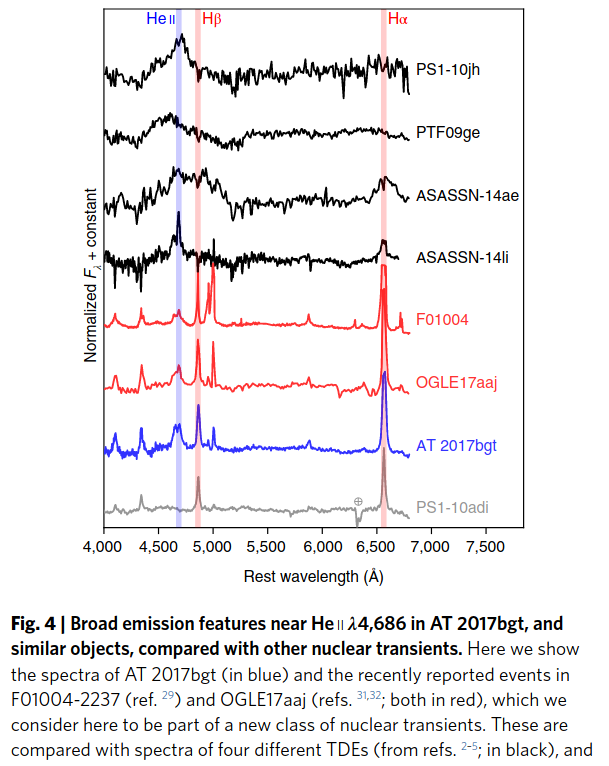
\includegraphics{/home/liuxing/git/Astro101/weekly_news/20210125-27/T19_nature-astro_fig4.png}
  \item
    2.He II 和 He I λ5876
    的宽度(FWHM,EW)逐渐变小,符合在其它TDE候选体中观察到的行为,而不符合在AGN中观察到的行为:随着光度减小,线宽增大。\\
    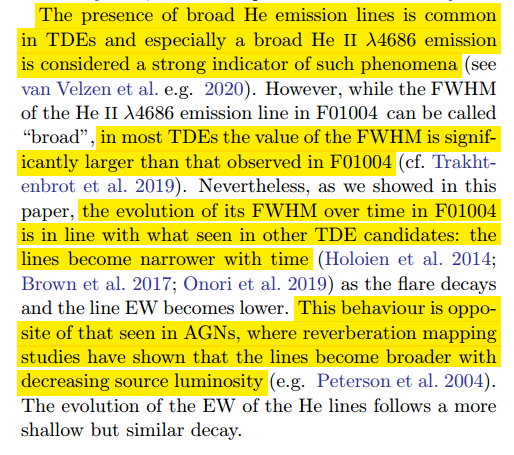
\includegraphics{/home/liuxing/git/Astro101/weekly_news/20210125-27/2101.09694_sa2.png}

    \begin{itemize}
    \item
      He线宽度的变化由中心黑动吸积流的变化导致。\\
      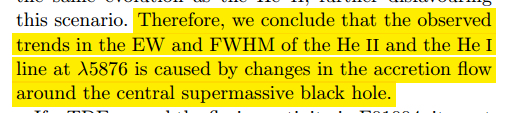
\includegraphics{/home/liuxing/git/Astro101/weekly_news/20210125-27/2101.09694_sa3.png}
    \end{itemize}
  \end{itemize}
\item
  T19 反对TDE解释的理由:

  \begin{itemize}
  \item
    持续时间长,He II线不够宽\\
    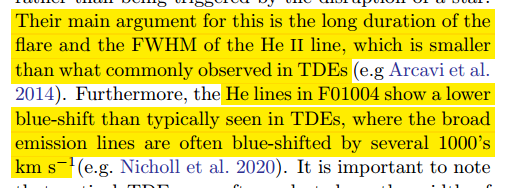
\includegraphics{/home/liuxing/git/Astro101/weekly_news/20210125-27/2101.09694_sa4.png}
  \item
    关于持续时间长(\textasciitilde10yr),本文作者认为可能是受到F01004中的AGN的影响。\\
    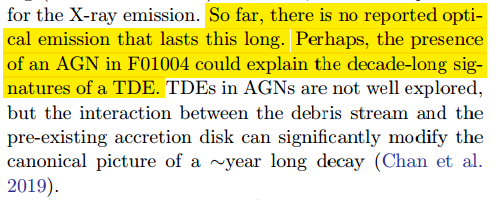
\includegraphics{/home/liuxing/git/Astro101/weekly_news/20210125-27/2101.09694_sa5.png}
  \end{itemize}
\end{itemize}

\begin{figure}
\centering
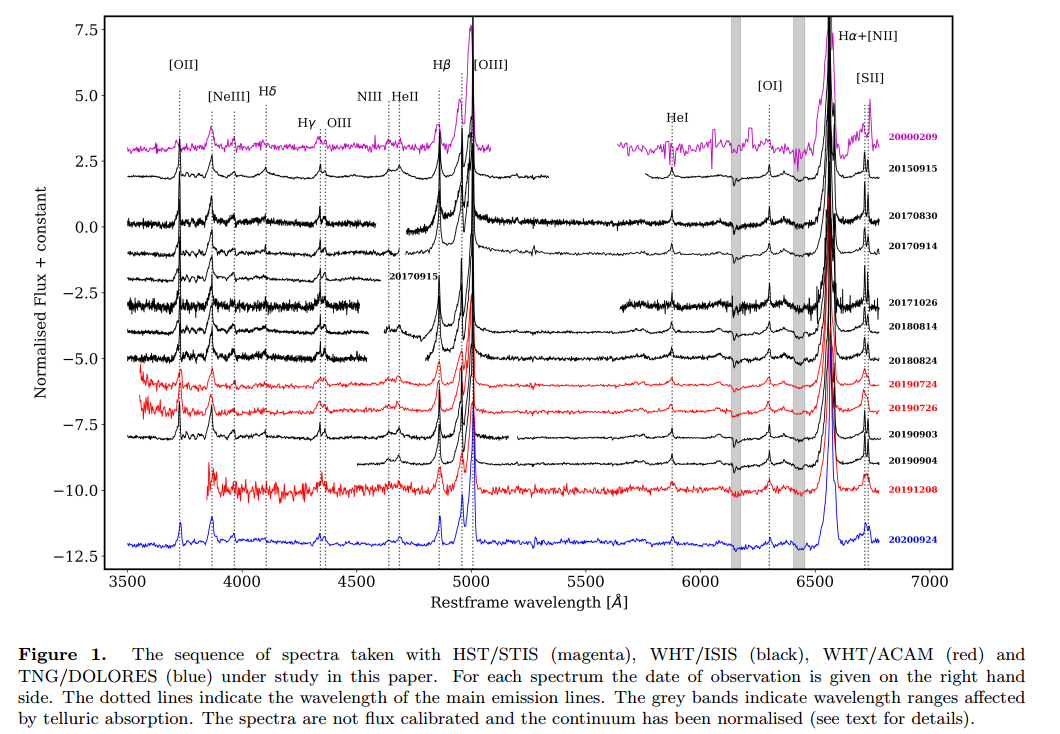
\includegraphics{/home/liuxing/git/Astro101/weekly_news/20210125-27/2101.09694_fig1.png}
\caption{}
\end{figure}

\begin{itemize}
\item
  AGN的光谱特征:

  \begin{itemize}
  \item
    \textbf{{[}O II{]} λ3727, {[}Ne III{]}λ3869, Hδ, Hγ, {[}O III{]}
    λ4363,λ4959,λ5007}, N III λ4640, He II λ4686, \textbf{Hβ, He I
    λ3889,λ5876, {[}O I{]} λ6300, Hα, {[}N II{]} λ6548,λ6584 and {[}S
    II{]} λ6717,6731}\\
    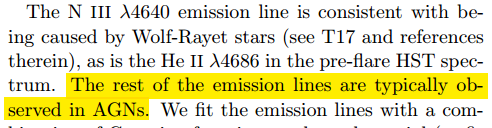
\includegraphics{/home/liuxing/git/Astro101/weekly_news/20210125-27/2101.09694_sa6.png}
  \end{itemize}
\end{itemize}

\hypertarget{header-n69}{%
\subsubsection{\texorpdfstring{\href{./2101.10581.pdf}{Off-axis jet
scenario for early afterglow emission of low-luminosity gamma-ray burst
GRB
190829A}}{Off-axis jet scenario for early afterglow emission of low-luminosity gamma-ray burst GRB 190829A}}\label{header-n69}}

https://arxiv.org/abs/2101.10581

details

Authors: Yuri Sato, Kaori Obayashi, Ryo Yamazaki, Kohta Murase, Yutaka
Ohira\\
Comments: 9 pages, 4 figures

Recently, ground-based Imaging Atmospheric Cherenkov Telescopes have
reported the detection of very-high-energy (VHE) gamma rays from some
gamma-ray bursts (GRBs). One of them, GRB\textasciitilde190829A, was
triggered by the Swift satellite, and about 20000 s after the burst
onset the VHE gamma-ray emission was detected by H.E.S.S. with
\textasciitilde{} 5 sigma significance. This event had unusual features
of having much smaller isotropic equivalent gamma-ray energy than
typical long GRBs and achromatic peaks in X-ray and optical afterglow at
about 1400 s. Here we propose an off-axis jet scenario that explains
these observational results. In this model, the relativistic beaming
effect is responsible for the apparently small isotropic gamma-ray
energy and spectral peak energy. Using a jetted afterglow model, we find
that the narrow jet, which has the initial Lorentz factor of 350 and the
initial jet opening half-angle of 0.015 rad, viewed off-axis can
describe the observed achromatic behavior in the X-ray and optical
afterglow. Another wide, baryon-loaded jet is necessary for the
later-epoch X-ray and radio emissions. According to our model, the VHE
gamma rays observed by H.E.S.S. at 20000 s may come from the narrow jet
through the synchrotron self-Compton process.

\begin{itemize}
\item
  GRB 190829A
  是由Swift触发的一个长爆,且在爆后\textasciitilde20000s,H.E.S.S探测到超高能的伽玛射线。
\item
  该爆主要特征是,其各向同性能量相对典型长爆来说很低,另外,X波段和光学波段的消色差拐折发生在大约1400s。
\item
  作者提出偏轴模型来解释观测特征:

  \begin{itemize}
  \item
    相对论集束效应导致看上去很小的各向同性能量,并且也能解释谱峰值能量。
  \item
    \(\Gamma_0 \sim 350\),
    \(\theta_0 \sim 0.015rad (0.86^{\circ})\)的狭窄喷流的偏轴观测可描述X射线和光学余辉的拐折。
  \item
    H.E.S.S在\textasciitilde20000s观测到的VHE伽玛射线可能来自喷流中的SSC过程。
  \end{itemize}
\end{itemize}

\begin{center}\rule{0.5\linewidth}{0.5pt}\end{center}

\begin{itemize}
\item
  VHE \(E_{\gamma}?\)
\item
  该事件的\(E_{iso}\)与典型长爆的\(E_{iso}\)?
\item
  20000s内有持续辐射?就光变曲线来看,应该是的。
\item
  偏轴如何解释\textasciitilde1400s的拐折?
\item
  跟踪观测情况?这篇文章应该没有自己观测,用的其他工作的数据。
\end{itemize}

\begin{center}\rule{0.5\linewidth}{0.5pt}\end{center}

\begin{itemize}
\item
  该事件的\(E_{iso}\)与典型长爆的\(E_{iso}\)?\\
  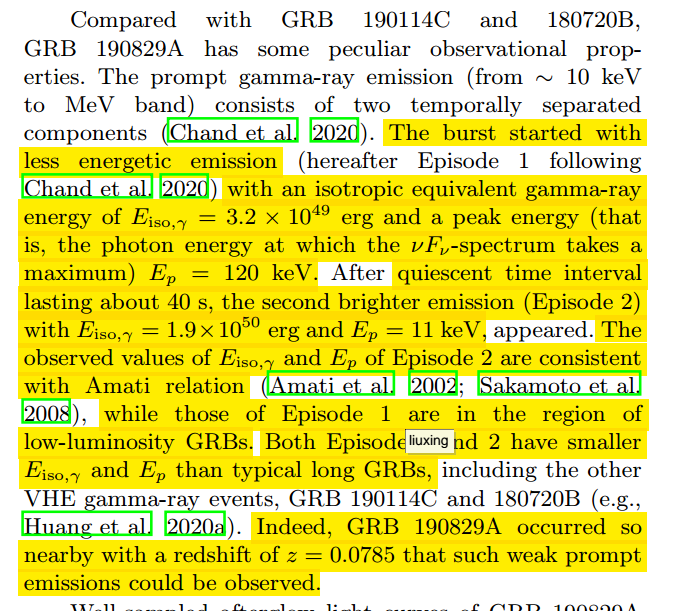
\includegraphics{/home/liuxing/git/Astro101/weekly_news/20210125-27/2101_10581_sa1.png}

  \begin{itemize}
  \item
    典型长爆大概在\(10^{51~55} erg\),量级53左右。来自韶宇学长的统计。
  \end{itemize}
\item
  20000s内有持续辐射?就光变曲线来看,应该是的。\\
  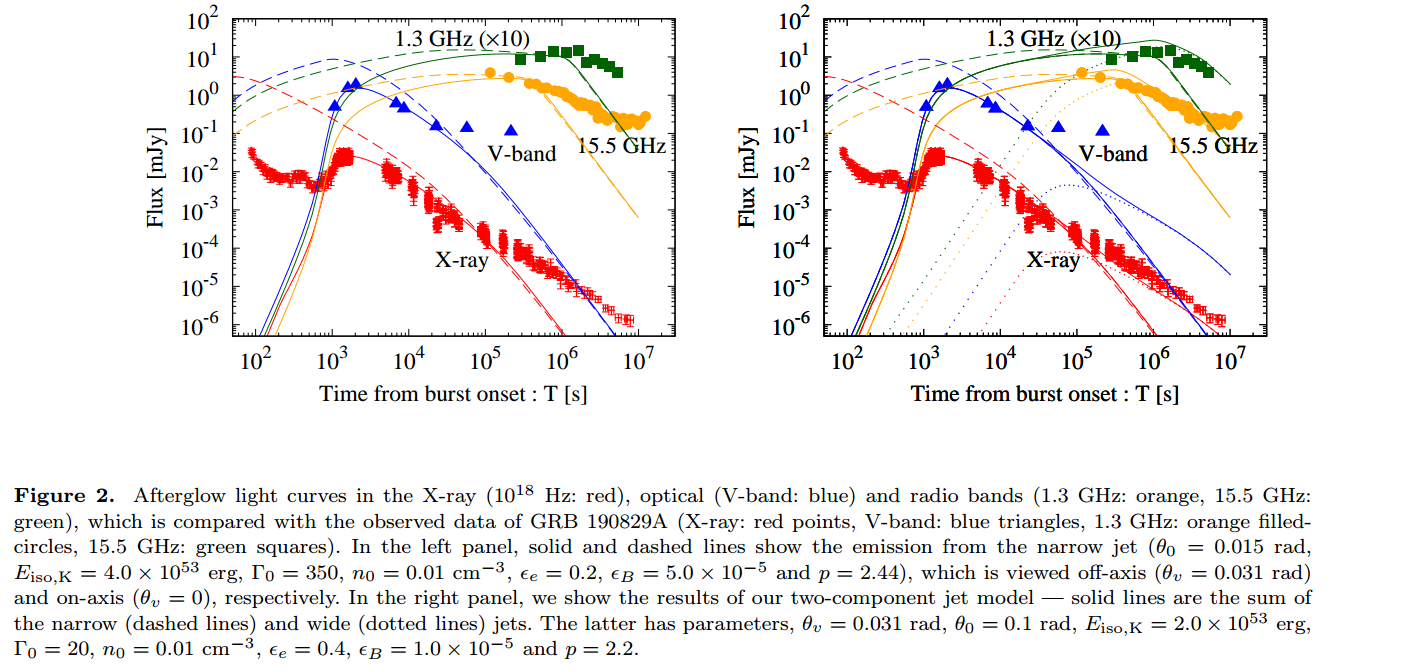
\includegraphics{/home/liuxing/git/Astro101/weekly_news/20210125-27/2101_10581_fig2.png}
\item
  跟踪观测情况?这篇文章应该没有自己观测,用的其他工作的数据。\\
  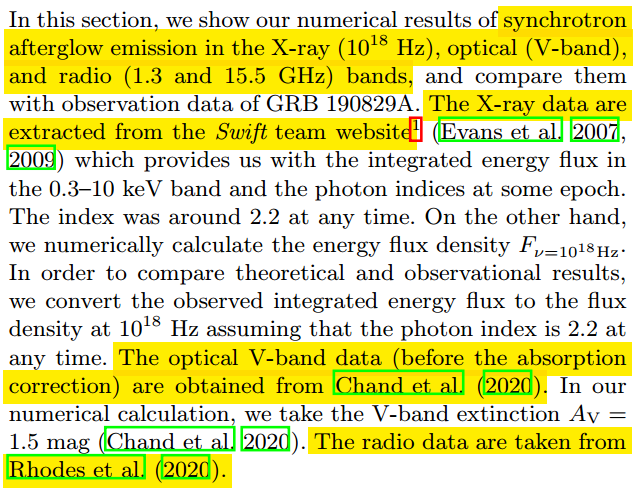
\includegraphics{/home/liuxing/git/Astro101/weekly_news/20210125-27/2101_10581_sa2.png}
\item
  偏轴如何解释\textasciitilde1400s的拐折?

  \begin{itemize}
  \item
    使用了双喷流模型,原因?\\
    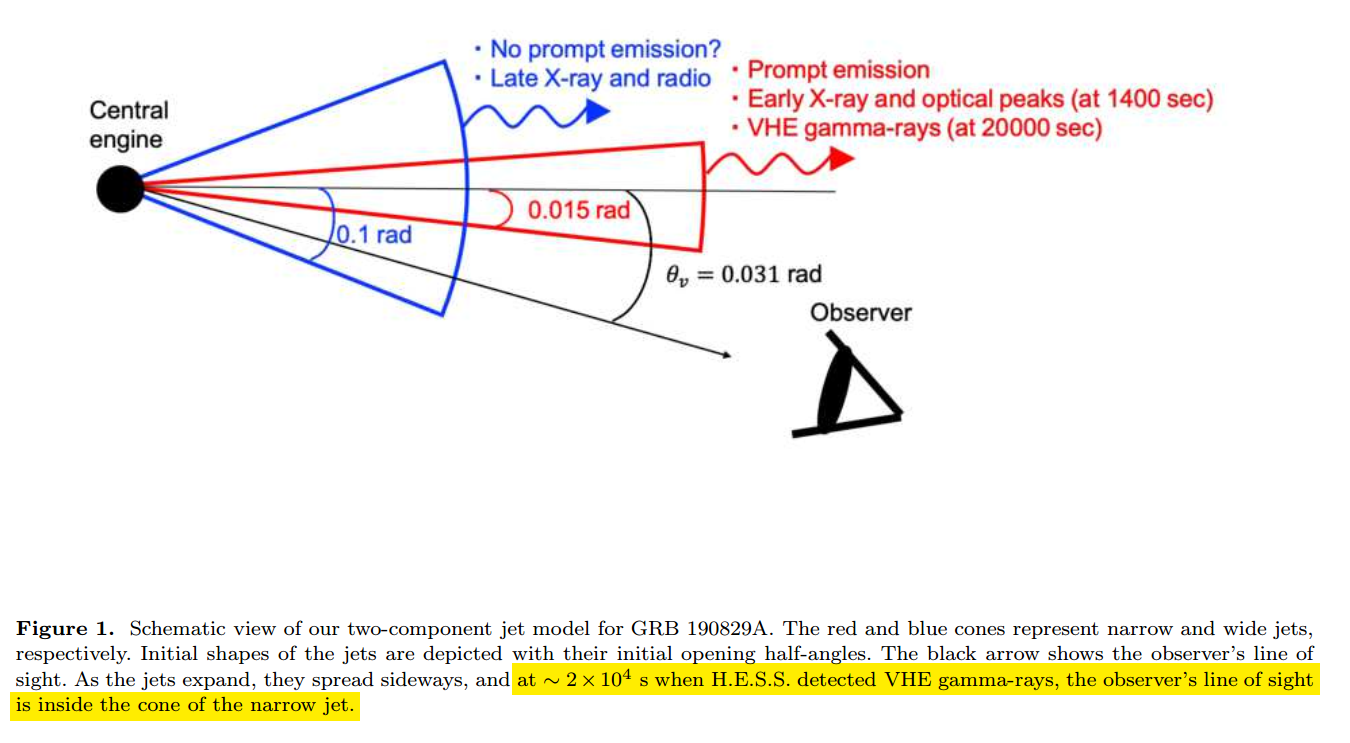
\includegraphics{/home/liuxing/git/Astro101/weekly_news/20210125-27/2101_10581_fig1.png}

    \begin{itemize}
    \item
      窄喷流成分主要解释~1400s的X射线和光学余辉的拐折\\
      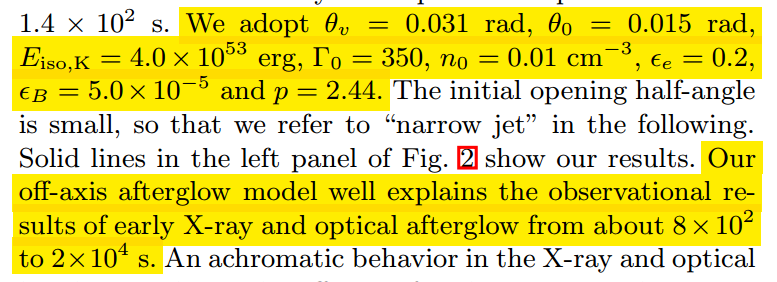
\includegraphics{/home/liuxing/git/Astro101/weekly_news/20210125-27/2101_10581_sa3.png}
    \item
      宽成分主要解释后期的射电和X射线光变\\
      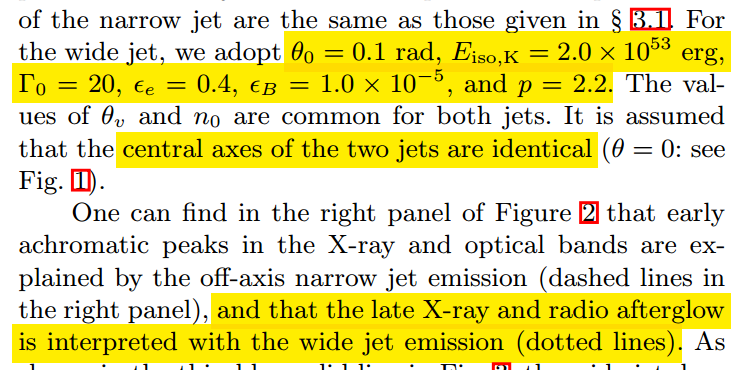
\includegraphics{/home/liuxing/git/Astro101/weekly_news/20210125-27/2101_10581_sa4.png}
    \item
      双成分瞬时辐射,\href{Chand_2020_ApJ_898_42.pdf}{Chand,2020},\href{https://iopscience.iop.org/article/10.3847/1538-4357/ab9606/pdf}{url}
    \end{itemize}
  \end{itemize}
\item
  VHE \(E_{\gamma}?\)\\
  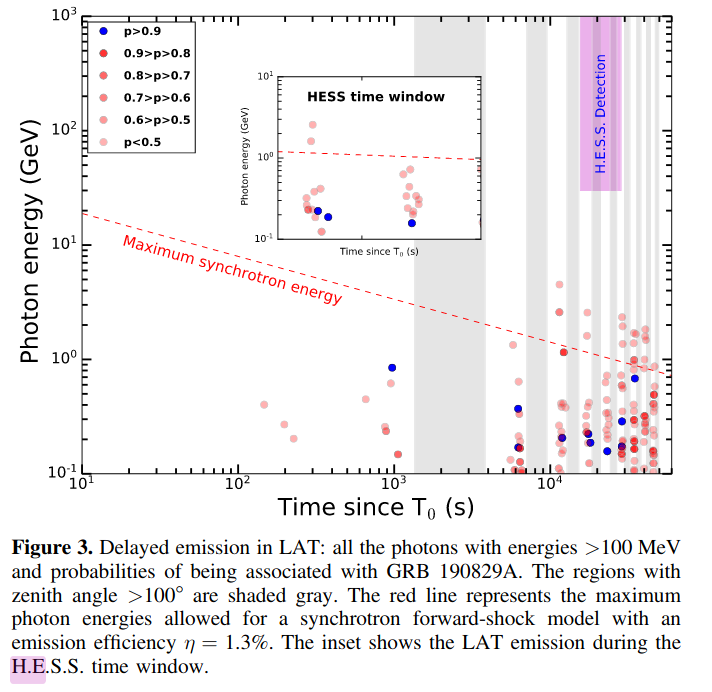
\includegraphics{/home/liuxing/git/Astro101/weekly_news/20210125-27/Chand_fig3.png}
\end{itemize}

\begin{figure}
\centering
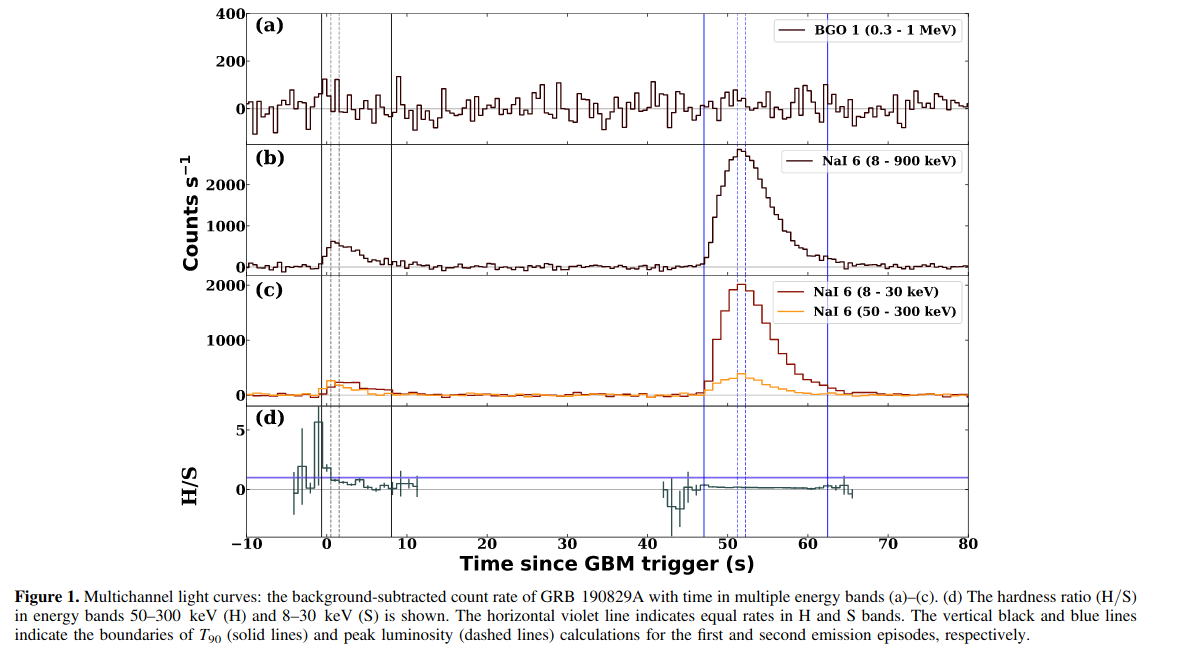
\includegraphics{/home/liuxing/git/Astro101/weekly_news/20210125-27/Chand_fig1.png}
\caption{}
\end{figure}

\hypertarget{header-n127}{%
\subsubsection{\texorpdfstring{\href{./2101.09430.pdf}{The fast evolving
type Ib Supernova SN 2015dj in NGC
7371}}{The fast evolving type Ib Supernova SN 2015dj in NGC 7371}}\label{header-n127}}

https://arxiv.org/abs/2101.09430

details

Authors: Mridweeka Singh, Kuntal Misra, Stefano Valenti, et al.\\
Comments: 16 pages, 11 figures, accepted for publication in ApJ

We present the detailed optical evolution of a type Ib SN 2015dj in NGC
7371, using data spanning up to ∼ 170 days after discovery. SN 2015dj
shares similarity in light curve shape with SN 2007gr and peaks at MV =
−17.37±0.02 mag. Analytical modelling of the quasi bolometric light
curve yields 0.06±0.01 M⊙ of 56Ni, ejecta mass Mej=1.4+1.3−0.5 M⊙, and
kinetic energy Ek=0.7+0.6−0.3×1051 erg. The spectral features show a
fast evolution and resemble those of spherically symmetric ejecta. The
analysis of nebular phase spectral lines indicate a progenitor mass
between 13-20 M⊙ suggesting a binary scenario.

\begin{itemize}
\item
  讨论了Ib型 SN2015dj (宿主星系NGC7371,\(D_L = 36.69\pm 0.05 Mpc\),
  \(z=0.0090\)) 直到发现后170天的光学波段演化。
\item
  其光变曲线与 SN2007gr 相似,峰值星等\(M_V = -17.32\pm 0.02\) mag。
\item
  准热光变曲线的模型拟合给出 56Ni:\(0.06\pm 0.01 M_⊙\),
  \(M_{ej} = 1.4^{+1.3}_{-0.5} M_⊙\),
  \(E_K =0.7^{+0.6}_{-0.3} \times 10^{51} erg\)。
\item
  光谱特征演化较快,与球对称外流情形相似。
\item
  星云阶段谱线分析显示前身星质量为13-20\(M_⊙\),有可能是一个双星。
\end{itemize}

\begin{center}\rule{0.5\linewidth}{0.5pt}\end{center}

\begin{itemize}
\item
  如何发现?跟踪观测情况?如何证认为Ib型SN?
\item
  如何与SN2007gr相似,有何含义?
\item
  如何计算准热光度?
\item
  哪些光谱特征演化较快?外流形状如何影响光谱演化?
\item
  如何分析星云阶段光谱?
\item
  为何13-20 M⊙ suggests 双星前身星而不是大质量恒星?
\end{itemize}

\begin{center}\rule{0.5\linewidth}{0.5pt}\end{center}

\begin{itemize}
\item
  发现与证认\\
  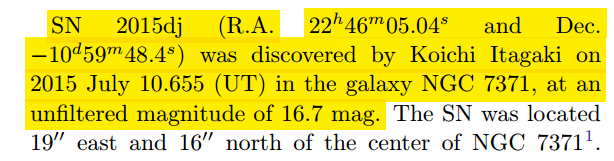
\includegraphics{/home/liuxing/git/Astro101/weekly_news/20210125-27/2101.09430_sa1.png}\\
  \href{http://www.cbat.eps.harvard.edu/unconf/followups/J22460504-1059484.html}{see
  reference}

  \begin{itemize}
  \item
    开始认为是IIb型超新星,后来分类为Ib型。\\
    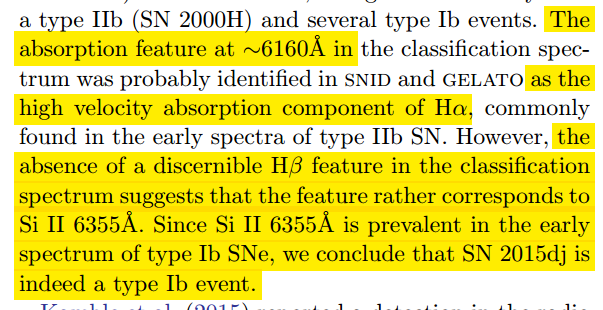
\includegraphics{/home/liuxing/git/Astro101/weekly_news/20210125-27/2101.09430_sa2.png}
  \end{itemize}
\item
  跟踪观测情况,see table1 and table2\\
  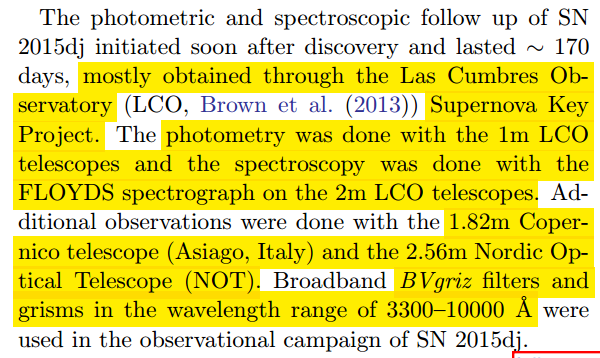
\includegraphics{/home/liuxing/git/Astro101/weekly_news/20210125-27/2101.09430_sa3.png}
\item
  see data reduction section\\
  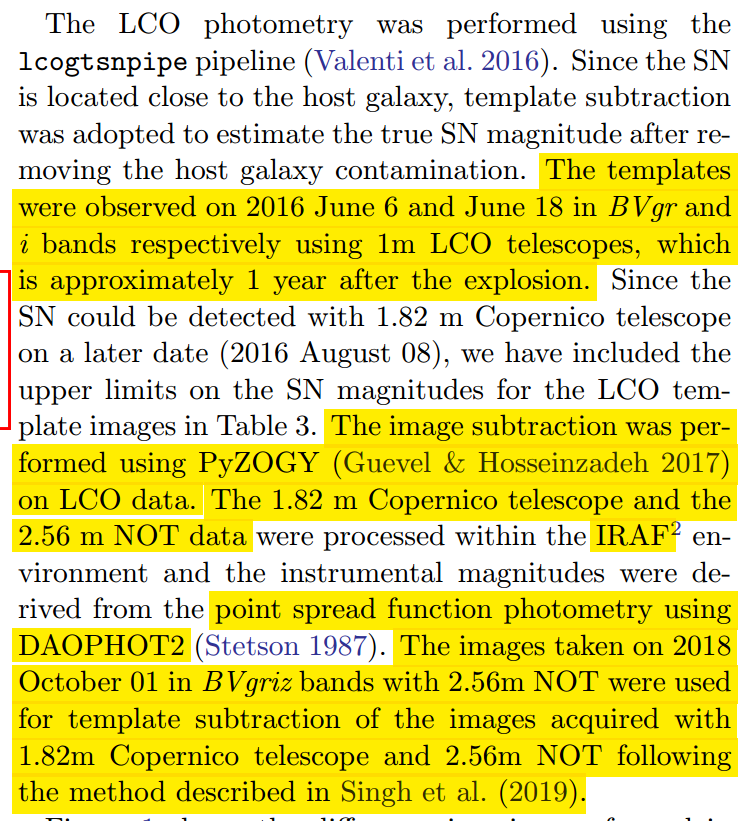
\includegraphics{/home/liuxing/git/Astro101/weekly_news/20210125-27/2101.09430_dr.png}

  \begin{itemize}
  \item
    提到了一个图像相减的python包\href{https://github.com/dguevel/PyZOGY}{PyZOGY},\href{Zackay_image-sub.pdf}{原理},方法有别与Alard\&Lupton,值得研究一下。
  \item
    最后说到的Singh et al.
    (2019)这篇\href{Singh_2019.pdf}{文章}没有提到如何做图像相减。
  \end{itemize}
\item
  与SN2007gr光变曲线的整体趋势都相似,没有提到有何含义\\
  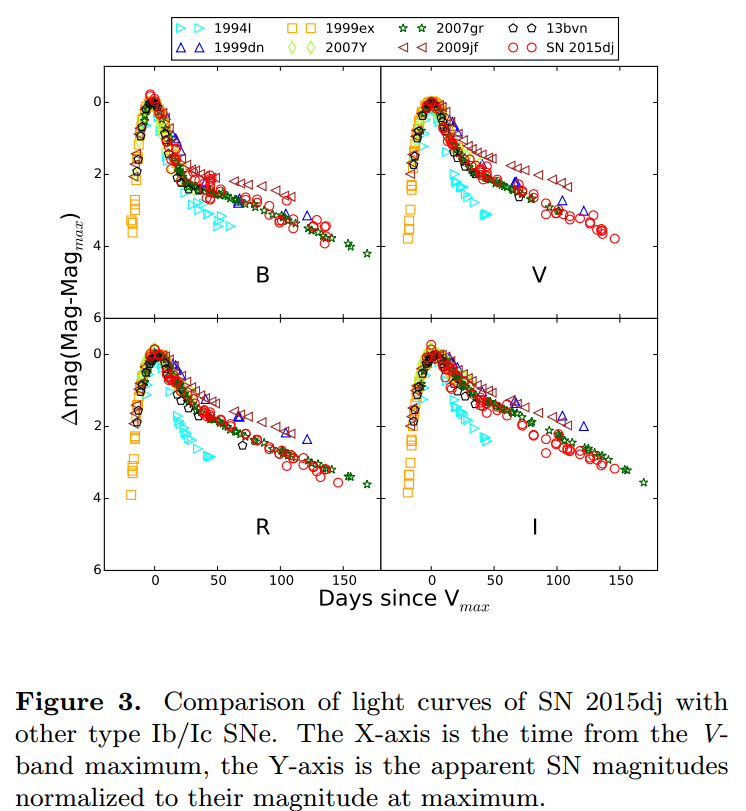
\includegraphics{/home/liuxing/git/Astro101/weekly_news/20210125-27/2101.09430_fig3.png}
\item
  使用BVRI波段星等计算准热光变曲线\\
  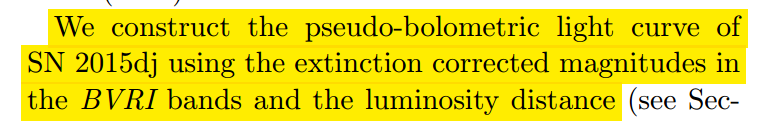
\includegraphics{/home/liuxing/git/Astro101/weekly_news/20210125-27/2101.09430_sa5.png}
\item
  星云阶段谱线无偏-\textgreater 球对称外流。即外流形状会影响谱线红移或蓝移\\
  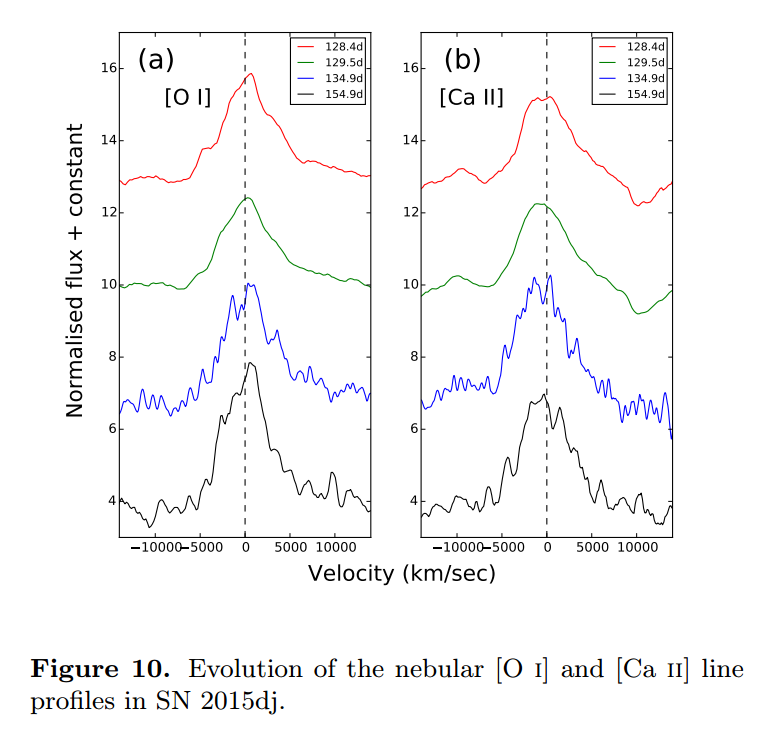
\includegraphics{/home/liuxing/git/Astro101/weekly_news/20210125-27/2101.09430_fig10.png}\\
  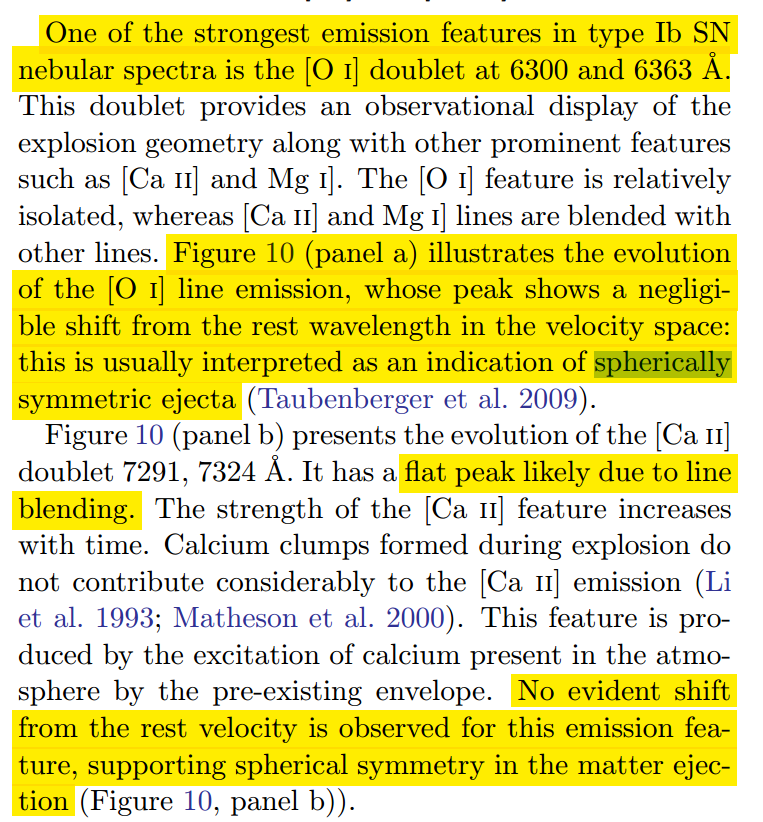
\includegraphics{/home/liuxing/git/Astro101/weekly_news/20210125-27/2101.09430_sa4.png}

  \begin{itemize}
  \item
    偏移谱线的例子:\href{2101.11340.pdf}{2101.11340}\\
    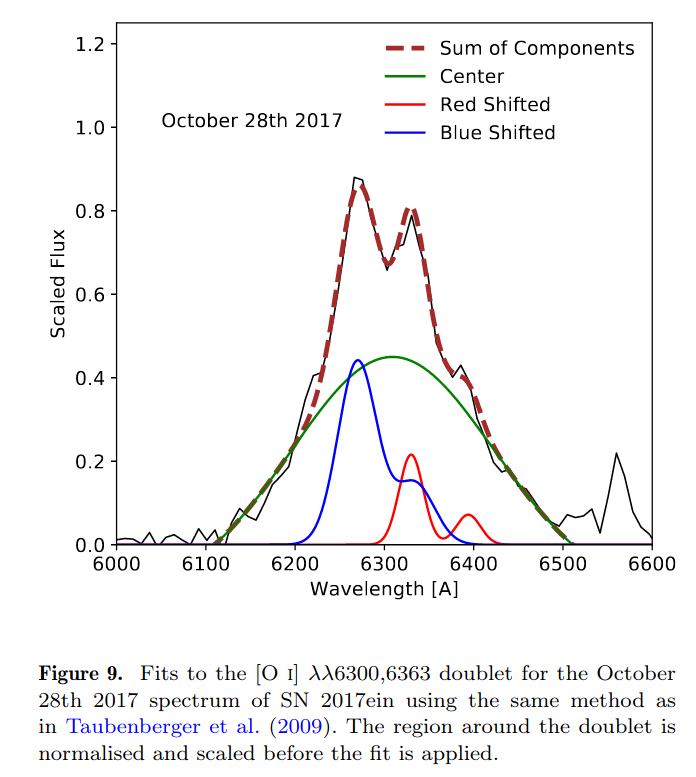
\includegraphics{/home/liuxing/git/Astro101/weekly_news/20210125-27/2101.11340_fig9.png}\\
    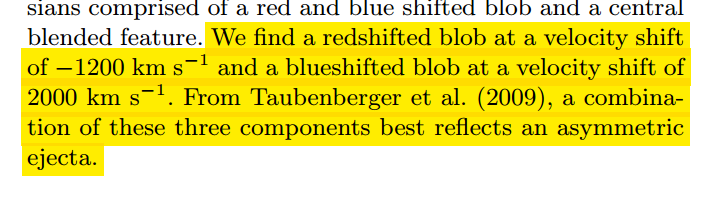
\includegraphics{/home/liuxing/git/Astro101/weekly_news/20210125-27/2101.11340_sa1.png}
  \item
    由此看似乎本文的判断不够严谨。
  \end{itemize}
\item
  由星云阶段 O I线推断前身星质量为15-20\(M_⊙\)\\
  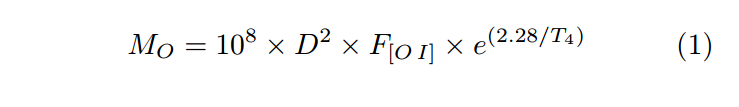
\includegraphics{/home/liuxing/git/Astro101/weekly_news/20210125-27/2101.09430_sa61.png}

  \begin{center}\rule{0.5\linewidth}{0.5pt}\end{center}

  \begin{figure}
  \centering
  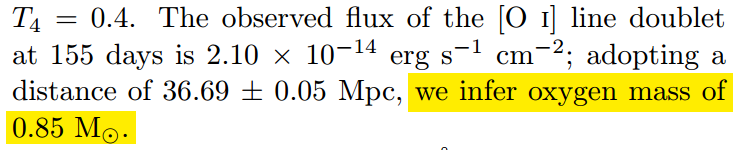
\includegraphics{/home/liuxing/git/Astro101/weekly_news/20210125-27/2101.09430_sa62.png}
  \caption{}
  \end{figure}

  \begin{center}\rule{0.5\linewidth}{0.5pt}\end{center}

  \begin{figure}
  \centering
  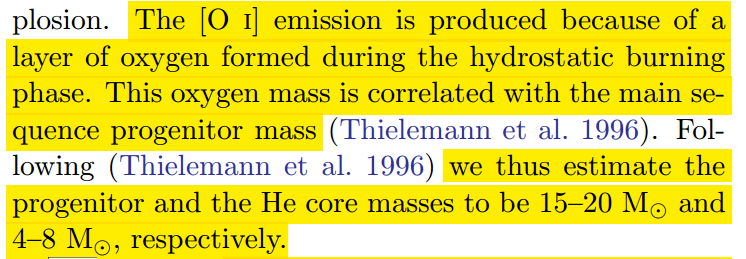
\includegraphics{/home/liuxing/git/Astro101/weekly_news/20210125-27/2101.09430_sa63.png}
  \caption{}
  \end{figure}
\item
  另一方面,经过与不同前身质量的核合成模型比较,显示该SN前身星质量约为13\(M_⊙\),故得出13-20\(M_⊙\)\\
  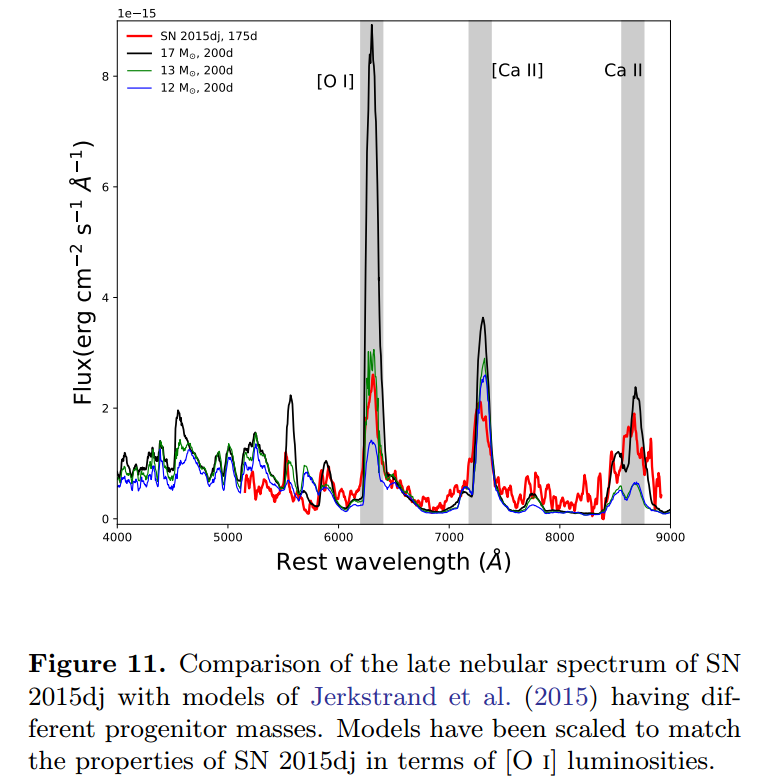
\includegraphics{/home/liuxing/git/Astro101/weekly_news/20210125-27/2101.09430_fig11.png}\\
  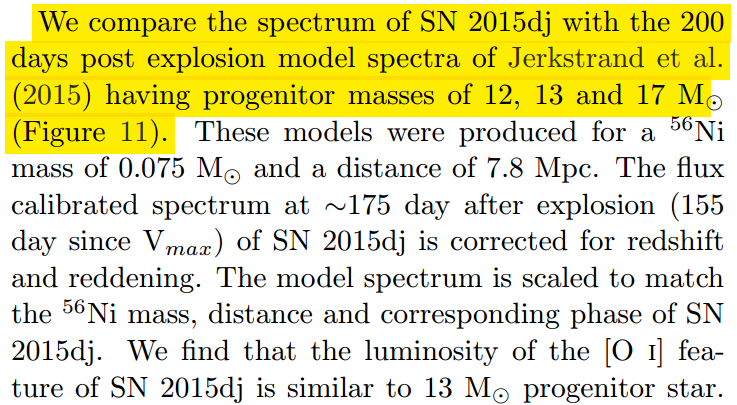
\includegraphics{/home/liuxing/git/Astro101/weekly_news/20210125-27/2101.09430_sa7.png}
\item
  为何认为是双星前身星?\\
  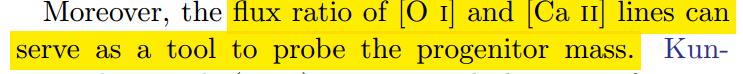
\includegraphics{/home/liuxing/git/Astro101/weekly_news/20210125-27/2101.09430_sa81.png}

  \begin{center}\rule{0.5\linewidth}{0.5pt}\end{center}

  \begin{figure}
  \centering
  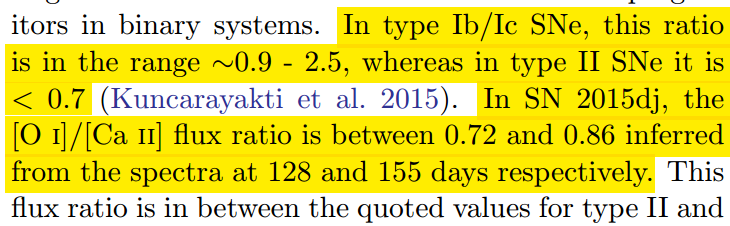
\includegraphics{/home/liuxing/git/Astro101/weekly_news/20210125-27/2101.09430_sa82.png}
  \caption{}
  \end{figure}

  \begin{center}\rule{0.5\linewidth}{0.5pt}\end{center}

  \begin{figure}
  \centering
  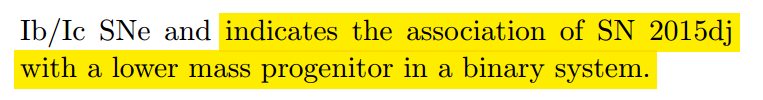
\includegraphics{/home/liuxing/git/Astro101/weekly_news/20210125-27/2101.09430_sa83.png}
  \caption{}
  \end{figure}

  \begin{itemize}
  \item
    为何质量在这之间的是双星?
    \href{Kuncarayakti_2015.pdf}{Kuncarayakti\_2015}\\
    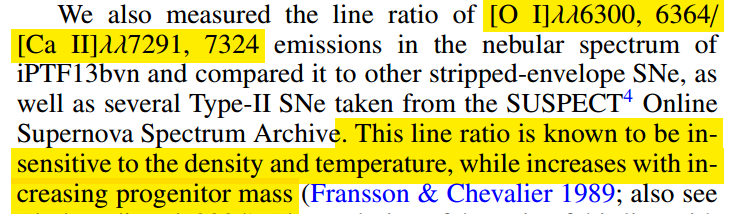
\includegraphics{/home/liuxing/git/Astro101/weekly_news/20210125-27/K15_sa1.png}

    \begin{center}\rule{0.5\linewidth}{0.5pt}\end{center}

    \begin{figure}
    \centering
    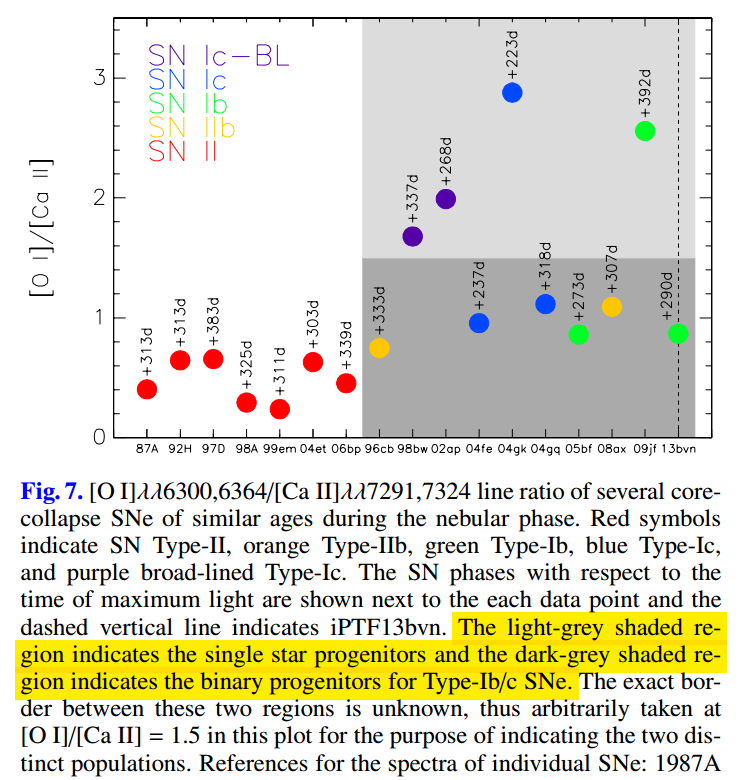
\includegraphics{/home/liuxing/git/Astro101/weekly_news/20210125-27/K15_fig7.png}
    \caption{}
    \end{figure}

    \begin{center}\rule{0.5\linewidth}{0.5pt}\end{center}

    \begin{figure}
    \centering
    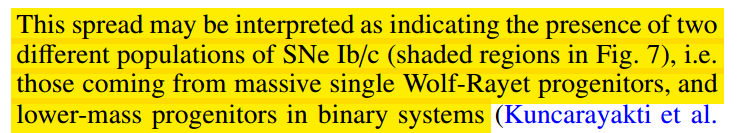
\includegraphics{/home/liuxing/git/Astro101/weekly_news/20210125-27/K15_sa2.png}
    \caption{}
    \end{figure}
  \end{itemize}
\end{itemize}

\hypertarget{header-n207}{%
\subsubsection{\texorpdfstring{\href{./2101.09792.pdf}{Exploring the
diversity of double detonation explosions for type Ia supernovae:
Effects of the post-explosion helium shell
composition}}{Exploring the diversity of double detonation explosions for type Ia supernovae: Effects of the post-explosion helium shell composition}}\label{header-n207}}

https://arxiv.org/abs/2101.09792

details

Authors: M. R. Magee, K. Maguire, R. Kotak, S. A. Sim\\
Comments: 21 pages, 25 figures, 1 table. Accepted for publication in
MNRAS. Model light curves available at
\href{https://github.com/MarkMageeAstro/TURTLS-Light-curves}{this https
URL}

The detonation of a helium shell on top of a carbon-oxygen white dwarf
has been argued as a potential explosion mechanism for type Ia
supernovae (SNe\textasciitilde Ia). The ash produced during helium shell
burning can lead to light curves and spectra that are inconsistent with
normal SNe\textasciitilde Ia, but may be viable for some objects showing
a light curve bump within the days following explosion. We present a
series of radiative transfer models designed to mimic predictions from
double detonation explosion models. We consider a range of core and
shell masses, and systematically explore multiple post-explosion
compositions for the helium shell. We find that a variety of
luminosities and timescales for early light curve bumps result from
those models with shells containing 56Ni, 52Fe, or 48Cr. Comparing our
models to SNe\textasciitilde Ia with light curve bumps, we find that
these models can reproduce the shapes of almost all of the bumps
observed, but only those objects with red colours around maximum light
(B−V≳1) are well matched throughout their evolution. Consistent with
previous works, we also show that those models in whichi the shell does
not contain iron-group elements provide good agreement wth normal
SNe\textasciitilde Ia of different luminosities from shortly after
explosion up to maximum light. While our models do not amount to
positive evidence in favour of the double detonation scenario, we show
that provided the helium shell ash does not contain iron-group elements,
it may be viable for a wide range of normal SNe\textasciitilde Ia.

考虑不同的核质量和壳层质量,以及一系列不同的壳层化学成分,可以模拟出不同的双爆轰情形下的超新星光变。(有bump的,普通的)

\begin{figure}
\centering
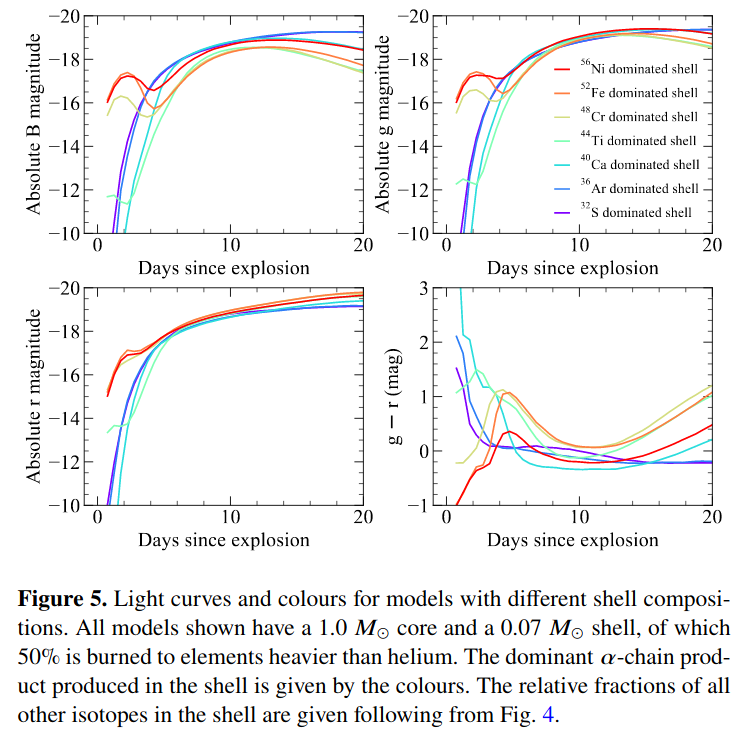
\includegraphics{/home/liuxing/git/Astro101/weekly_news/20210125-27/2101.09792_fig5.png}
\caption{}
\end{figure}

\end{document}
